\documentclass{beamer}
%Information to be included in the title page:
\title{Étude de la chute de Phobos sur Mars}
\author{Armand et Nathan}
\date{2026}

\begin{document}
	
	\frame{\titlepage}
	
	\begin{frame}{Modélisation du retard de marée}
		
		\begin{minipage}{0.54\textwidth}
			\centering
			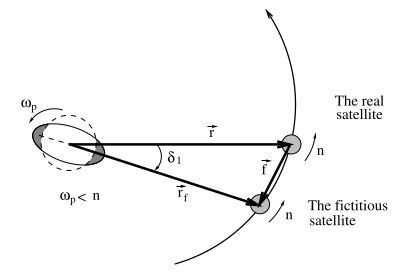
\includegraphics[scale=.43]{Image/shema_planete.png}
			
			\vspace{0.15cm}
			{\scriptsize Schéma du décalage de marée}
		\end{minipage}
		\hfill
		\begin{minipage}{0.42\textwidth}
			
			{\scriptsize \textbf{Grandeurs introduites}}
			
			\vspace{-0.1cm}
			
			{\scriptsize
				\begin{itemize}
					\item $\mathbf r$ : position du satellite
					\item $\mathbf r_f$ : satellite fictif
					\item $\mathbf f$ : retard spatial
					\item $\Delta t$ : retard temporel
					\item $\boldsymbol{\omega}_p$ : rotation de la planète
					\item $\mathbf v$ : vitesse du satellite
					\item $n$ : vitesse angulaire orbitale
					\item $\delta$ : retard angulaire
					\item $\chi$ : fréquence principale de marée
				\end{itemize}
			}
			
			\vspace{0.05cm}
			
			{\small \textbf{Relations principales}}
			\vspace{-0.2cm}
			\[
			\begin{aligned}
				\mathbf r_f &= \mathbf r+\mathbf f,\\[0.15cm]
				\mathbf f &= \Delta t(\boldsymbol{\omega}_p\times\mathbf r-\mathbf v),\\[0.15cm]
				\delta &\approx \frac{|\mathbf f|}{r}
				= \frac{\Delta t}{2}\chi,\\[0.15cm]
				\chi &= 2|\omega_p-n|.
			\end{aligned}
			\]
			
		\end{minipage}
		
	\end{frame}
	
	\begin{frame}{Facteur de qualité du manteau planétaire}
		
		\small
		
		\textbf{Ancien modèle :}
		
		\[Q \sim \chi^{0}, \,\,\,\,\, 
		Q \sim \chi^{-1}
		\]
		
		\vspace{0.18cm}
		
		\textbf{Mesures sismologiques récentes :}
		
		\[
		Q \sim \chi^\alpha
		\]
		
		\[
		1\,\text{an}^{-1} \lesssim \chi \lesssim 10^7 \text{ Hz},
		\qquad
		0.2 \leq \alpha \leq 0.4
		\]
		
		\vspace{0.18cm}
		
		\textbf{Lien avec le retard de marée :}
		
		\[
		Q^{-1}\approx 2\delta
		\]
		
		\[
		\delta \approx \frac{\Delta t}{2}\chi
		\]
		
		\[
		\Delta t
		=
		\mathcal{E}^{\alpha}
		\chi^{-(\alpha+1)}
		\]
		
		\vspace{0.13cm}
		\textbf{À haute fréquence : réponse plus élastique du manteau}
		\[
		\chi \uparrow
		\quad \Rightarrow \quad
		Q \uparrow
		\quad \Rightarrow \quad
		\delta \downarrow
		\quad \Rightarrow \quad
		\Delta t \downarrow
		\]
	\end{frame}
	
	\begin{frame}{Obtention de l’équation sur le demi-grand axe}
		
		\small
		
		\textbf{Équation du mouvement :}
		
		\[
		\ddot{\mathbf r}
		=
		-\frac{G(M_0+m)}{r^3}\mathbf r
		+
		\mathbf F_{\text{marée}}
		\]
		
		\vspace{0.15cm}
		
		\textbf{Force de marée quadrupolaire :}
		
		\[
		\mathbf F_{\text{marée}}
		=
		-\frac{3k_2G(M_0+m)mR^5}{r^{10}M_0}
		\left[
		-\mathbf f\,r^2
		-
		2\mathbf r(\mathbf r\cdot\mathbf f)
		\right]
		\]
		
		\vspace{0.15cm}
		
		\textbf{Projection sur la composante tangentielle du mouvement :}
		
		
		\[
		\frac{da}{dt}
		=
		\frac{6k_2R^5nm\Delta t}{M_0a^4}(n-\omega_p)
		\]
		
		avec :
		
		\[
		\Delta t
		=
		\mathcal{E}^{\alpha}
		\left(2|n-\omega_p|\right)^{-(\alpha+1)}
		\]
		
		\[
		n(a)=\sqrt{\frac{GM_0}{a^3}}
		\]
		
	\end{frame}
	
	%NATHAN
	
	\begin{frame}
		\begin{center}
			\huge{\textbf{Résolution numérique}}
		\end{center}
	\end{frame}
	
	\begin{frame}{Objectifs de la résolution numérique}
		\begin{block}{}
			\begin{itemize}
				\item Étudier l'équation différentielle du demi-grand axe :
				\[
				\frac{da}{dt} = f(a) = -\frac{6k_2R^5mn(a)}{M_0a^4}\Delta t(a)(n(a) - \omega_p)
				\]
				\item Comparer les méthodes numériques :
				\begin{itemize}
					\item Euler explicite (ordre 1)
					\item Heun (ordre 2)
					\item Runge-Kutta 45 (référence)
				\end{itemize}
			\end{itemize}
		\end{block}
	\end{frame}
	
	\begin{frame}{Existence de la solution}
		
		\begin{center}
			EDO à résoudre : $\begin{cases}
				\dfrac{da}{dt} = f(a)\\
				a(0) = a_0
			\end{cases}$
			
			\vspace{.5cm}
			
			$\to$ $f$ est un "polynôme" rationnelle avec un unique pôle en 0.\pause
			
			\vspace{.5cm}
			
			$\to$ On arrêtera la résolution lorsque $a$ descend en dessous de $a_{min}$
		\end{center}
		
	\end{frame}
	
	% --- Page 2 ---
	\begin{frame}{Méthode d'Euler explicite}
		\begin{block}{\underline{Principe}}
			Schéma itératif : $a_{n+1} = a_n + h f(a_n)$
			
			$\to$ \textbf{Ordre 1} : Erreur en $O(h)$.
		\end{block}\pause
		
		\begin{block}{\underline{Analyse théorique}}
			\textbf{Erreur :}
			\[
			|a(t_n) - a_n| \leq e^{LT} \frac{M_2 T}{2} h
			\]\pause
			\begin{itemize}
				\item Pour $\alpha = 0.2$ : $|a(t_n) - a_n| \leq 2.96 \times 10^{-7} h$ \pause
				\item Exemple : Avec $h = 100$ ans et $T = 35$ Ma (400 000 points),
				\begin{center}
					erreur $\leq 931.7$ m.
				\end{center}
			\end{itemize}\pause
			
			\vspace{.2cm}
			
			\textbf{Erreur relative :} \begin{itemize}
				\item $Err_{rel} = \dfrac{\sup_n\lvert a(t_n)-a_n\rvert}{\sup_n\lvert a(t_n)\rvert} \leq e^{LT}\dfrac{M_2T}{2(a_0-\sup\lvert f \rvert T)}h $\\
				\item Pour $\alpha = 0.2$, $Err_{rel} \leq 3,3\times10^{-14} h$
			\end{itemize}
		\end{block}
		
	\end{frame}
	
	\begin{frame}
		\begin{alertblock}{\underline{Plage de validité}}
			\begin{itemize}
				\item Arrêt à $a_{min} = a_{roche}$ : erreur maîtrisée.\pause
				\item Arrêt à $a_{min} = R$ : majoration inutilisable en pratique.
			\end{itemize}
		\end{alertblock}
	\end{frame}
	
	
	\begin{frame}{Comparaison avec Runge-Kutta 45}
		
		\begin{center}
			$Erreur = C \times h^{ordre}$
		\end{center}
		
		\begin{block}{Ordre de convergence pour $a_{min} = a_{roche}$}
			\begin{itemize}
				\item \textbf{Euler} :
				\begin{itemize}
					\item Ordre \textbf{1} confirmé (\textbf{0,995}) et de coefficient : $C = 3.08 \times 10^{-16}$.
					\item Temps de calcul pour $h = 100$ ans : \begin{minipage}[t]{3cm}
						\textbf{2 secondes} pour 350 000 itérations.
					\end{minipage}
				\end{itemize}\pause
				\item \textbf{Runge-Kutta 45} :
				\begin{itemize}
					\item Solution de référence pour valider Euler 
				\end{itemize}\pause
			\end{itemize}
		\end{block}
		
		\begin{alertblock}{Limites}
			Majoration théorique inutilisable pour $a_{min} = R$. \\
			\textbf{Mais}, en pratique, l'erreur reste acceptable : $C =4,4\times10^{-13}$
		\end{alertblock}
	\end{frame}
	
	% --- Page 3 ---
	\begin{frame}{Résultats avec Euler}
		\begin{block}{Évolution du demi-grand axe}
			
			\begin{itemize}
				\item Décroissance vers $a_{roche}$ en \textbf{26.2 millions d'années} ($\alpha = 0.2$).
			\end{itemize}
		\end{block}
		
		\begin{figure}
			\centering
			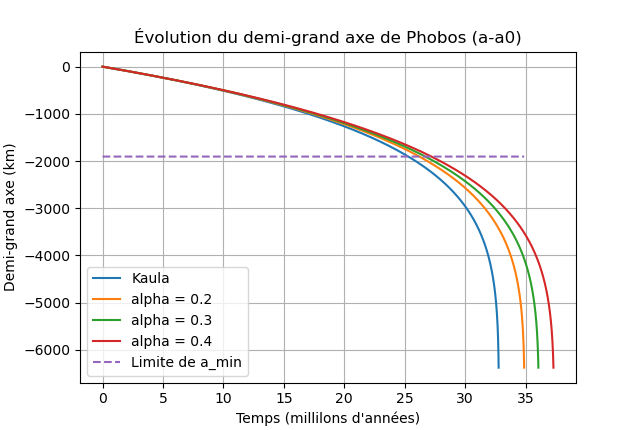
\includegraphics[width=0.8\textwidth]{Image/sol.png}
			\caption{Évolution du demi-grand axe de Phobos.}
		\end{figure}
	\end{frame}
	
	% --- Page 5 ---
	\begin{frame}{Méthode de Heun (Ordre 2)}
		\begin{block}{Principe}
			Schéma prédicteur-correcteur :
			\[
			a_{n+1} = a_n + \frac{h}{2} \left( f(a_n) + f(a_n + h f(a_n)) \right)
			\]
			$\to$ \textbf{Ordre 2} : Erreur en $O(h^2)$.
		\end{block}\pause
		
		\begin{block}{Analyse théorique}
			Erreur en norme infinie pour $ h \leq 10^{2}$ :
			\[
			|a(t_n) - a_n| \leq  e^{T\left(L+\dfrac{h_{max}L^2}2\right)}\dfrac{CT}{24}h^2 \simeq 3.28 \times 10^{-22} h^2 
			\]
			Erreur relative pour $ h \leq 10^{2}$ :
			\[
			\frac{\sup_n |a(t_n) - a_n|}{\sup_n |a(t_n)|} \leq 7.2 \times 10^{-29} 
			\]
		\end{block}
	\end{frame}
	
	% --- Page 6 ---
	\begin{frame}{Résultats, en pratique, avec Heun}
		
			\begin{center}
			$Erreur = C \times h^{ordre}$
		\end{center}
		
		\begin{block}{Comparaison avec Euler}
			\begin{itemize}
				\item \textbf{Ordre 2 confirmé (1,79)} :
				\begin{itemize}
					\item Coefficient : $C = 1.24 \times 10^{-29}$ ($a_{min} = a_{roche}$).
					\item \textbf{100 fois plus précis} qu'Euler pour un même pas.
				\end{itemize}\pause
				
				\vspace{.5cm}
				
				\item \textbf{Coût calcul} :
				\begin{itemize}
					\item \textbf{2 fois plus lent} (en moyenne : 1,96) qu'Euler.
					\item Mais : Pour un pas grossier ($h =$ 10 000 ans),\\
					     \hspace{1cm}Heun = précision d'Euler avec un pas fin ($h = 100$ ans).
				\end{itemize}
			\end{itemize}
		\end{block}\pause
		
		\begin{alertblock}{Limites}
			Majoration théorique inutilisable pour $a_{min} = R$. \\
			\textbf{Mais}, en pratique, l'erreur reste acceptable : $C =1,32\times10^{-27}$
		\end{alertblock}
	\end{frame}
	
	\begin{frame}{Graphique de la convergence}
		\begin{figure}
			\centering
			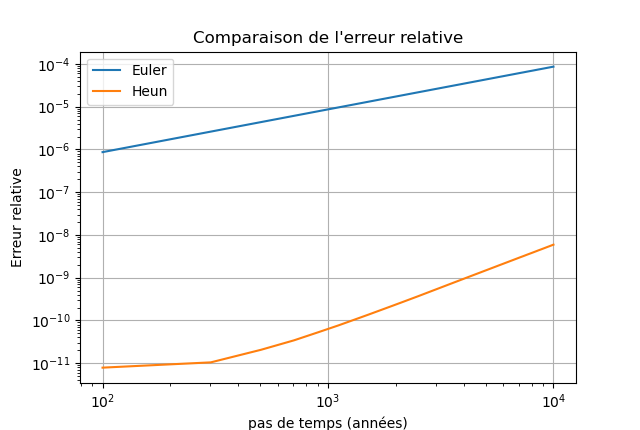
\includegraphics[width=0.8\textwidth]{Image/comparaison_erreur.png}
			\caption{Convergence en échelle log-log.}
		\end{figure}
	\end{frame}
	
	\begin{frame}{Graphique du temps de calcul}
		\begin{figure}
			\centering
			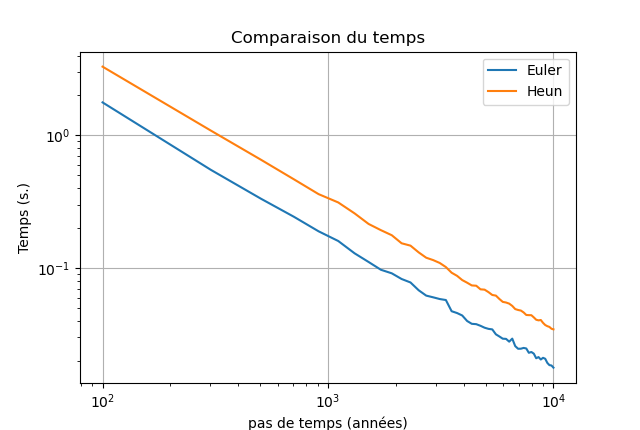
\includegraphics[width=0.8\textwidth]{Image/comparaison_temps.png}
			\caption{Convergence en échelle log-log.}
		\end{figure}
	\end{frame}
	
	% --- Page 7 ---
	\begin{frame}{Conclusion \& Perspectives}
		\begin{block}{Synthèse}
			
			\vspace{-.4cm}
			
		    \begin{table}
				\centering
				\begin{tabular}{|c|c|c|c|}
					\hline
					\textbf{Méthode} & \textbf{Ordre} & \textbf{Erreur} & \textbf{Temps calcul} \\
					\hline
					Euler & 1 & $\sim 10^{-7} h$ & Rapide \\
					Heun & 2 & $\sim 10^{-22} h^2$ & 2× plus lent \\
					Runge-Kutta 45 & 4/5 & Référence & - \\
					\hline
				\end{tabular}
			\end{table}
			\begin{itemize}
				\item \textbf{Heun} : Meilleur compromis précision/coût pour ce problème.
				\item \textbf{Limite} : Majoration théorique inutilisable près de $R$.
			\end{itemize}
		\end{block}
		
		\begin{block}{Perspectives}
			\begin{itemize}
				\item Tester d'autres méthodes.
				\item Affiner le modèle physique (ex : enlever des approximations comme $Q^{-1} = \tan 2\delta$).
				\item Le tester sur d'autres corps célestes.
			\end{itemize}
		\end{block}
	\end{frame}
\end{document}